\documentclass[11pt,a4paper]{beamer}
\usepackage[utf8]{inputenc}
%\usepackage[english]{babel}
\usepackage[T1]{fontenc}
\usepackage{amsmath}
\usepackage{amsthm}
\usepackage{amssymb}
\usepackage{amstext}

\usepackage[figurename = Obr., tablename = Tab.]{caption}

\setbeamertemplate{navigation symbols}{}

\usetheme		{Warsaw}%,Malmoe,Warsaw,3kolonky:CambridgeUS,Madrid %%Ilmenau,Antibes,,,,Luebeck,Copenhagen,
%\beamertemplateballitem
\usecolortheme	{orchid}%crane, orchid

\author{Bc. Jan Kučera}
\title{Robustnost Rényiho odhadů hustot pravděpodobnosti}
\institute{FJFI, ČVUT\\ $\quad$  \\ Vedoucí práce: Ing. Václav Kůs Ph.D.}
\date{6.9.2012}

\newcommand{\intpa}{\int p_\theta^{1+\alpha}(x) \, \mathrm{d}x }
\newcommand{\fn}{\frac{1}{n} \sum_{i=1}^n p_{\theta}^{\alpha}\left( x_i \right)}
\newcommand{\fln}{\frac{1}{n} \sum_{i=1}^n \ln p_{\theta}\left( x_i \right)}
\newcommand{\Cat}{C_\alpha\left( \theta \right)}
\newcommand{\amtiT}{\arg \max_{\theta \in \Theta}}
\newcommand{\fa}{\frac{\alpha}{1+\alpha}}


\begin{document}

\begin{frame}
	\maketitle
\end{frame}

\begin{frame}{Obsah}
    	\tableofcontents
\end{frame}

%
\begin{frame}{Značení}
\begin{description}
	\item[$\mathcal{P} = \lbrace P_\theta : \theta \in \Theta \subset \mathbb{R}^m \rbrace$] je množina distribučních funkcí na  $\left(\mathcal{X},\mathcal{A}\right)$ charakterizující použitý model
	\item[$X_1,\ldots,X_n$] je náhodný výběr z rozdělení $\tilde{P}$. Nepožadujeme, aby platilo $\tilde{P} \in \mathcal{P}$.
	\item[$\mathcal{\tilde{P}}$] = $\mathcal{P} \cup \lbrace \tilde{P} \rbrace$
\end{description}
\end{frame}

\section{Rozložitelné pseudovzdálenosti} %******************************************** PSEUDO-DISTANCE
\begin{frame}{Rozložitelné pseudovzdálenosti}
		Řekneme, že $\mathfrak{D}:\mathcal{P} \rightarrow \mathbb{R}$ je \emph{pseudovzdálenost}, pokud platí $\forall P,Q\in\mathcal{P}$
		\begin{equation*}
			\mathfrak{D}(P,Q) \geq 0  \qquad \text{a} \qquad \mathfrak{D}(P,Q)=0 \; \Leftrightarrow \; P=Q.
		\end{equation*}
		 Tato  pseudovzdálenost je  \emph{rozložitelná} pokud existují funkcionály
		 $\mathfrak{D}^0:\mathcal{P}\rightarrow\mathbb{R}$, $ \mathfrak{D}^1:\mathcal{\tilde{P}} \rightarrow \mathbb{R}$ a měřitelná
		  $\rho_\theta : \mathcal{X} \rightarrow \mathbb{R}$, $ \theta \in \Theta$ tak, že $\forall \theta \in \Theta$ a $\forall Q \in \mathcal{\tilde{P}}$ existuje konečná $\int{\rho_\theta }\mathrm{d}Q$ a
		\begin{equation*}
			\mathfrak{D} (P_\theta, Q) = \mathfrak{D}^0 (P_\theta) + \mathfrak{D}^1 (Q) + \int \rho_\theta \mathrm{d}Q.
		\end{equation*}

			Pozn.: Nepožadujeme trojúhelníkovou nerovnost, ani symetrii
		
\end{frame}

\begin{frame}{Rozložitelné pseudovzdálenosti}
		Řekneme, že $\mathfrak{D}:\mathcal{P} \rightarrow \mathbb{R}$ je \emph{pseudovzdálenost}, pokud platí $\forall P,Q\in\mathcal{P}$
		\begin{equation*}
			\mathfrak{D}(P,Q) \geq 0  \qquad \text{a} \qquad \mathfrak{D}(P,Q)=0 \; \Leftrightarrow \; P=Q.
		\end{equation*}
		 Tato  pseudovzdálenost je  \emph{rozložitelná} pokud existují funkcionály
		 $\mathfrak{D}^0:\mathcal{P}\rightarrow\mathbb{R}$, $ \mathfrak{D}^1:\mathcal{\tilde{P}} \rightarrow \mathbb{R}$ a měřitelná
		  $\rho_\theta : \mathcal{X} \rightarrow \mathbb{R}$, $ \theta \in \Theta$ tak, že $\forall \theta \in \Theta$ a $\forall Q \in \mathcal{\tilde{P}}$ existuje konečná $\int{\rho_\theta }\mathrm{d}Q$ a
		\begin{equation*}
			\mathfrak{D} (P_\theta, Q) ={\color{red} \mathfrak{D}^0 (P_\theta) }+ \mathfrak{D}^1 (Q) + {\color{red}\int \rho_\theta \mathrm{d}Q}.
		\end{equation*}
		Odhad s minimální vzdáleností {\color{red}minimalizuje}
\end{frame}

%\begin{frame}
%	\begin{itemize}
%		\item methods based on minimization of some functional
%		
%	\end{itemize}
%\end{frame}

%\begin{frame}{Odhady s minimální vzdáleností}
%	Funkcionál $T_\mathfrak{D}:\mathcal{\tilde{P}} \rightarrow \Theta$ definuje odhad s minimální vzdáleností, pokud  $\mathfrak{D}(P_\theta,Q)$ je rozložitelná a $T_\mathfrak{D}(Q) \in \Theta$ minimalizuje   
%	\begin{equation*}
%		T_\mathfrak{D}(Q) = \arg \min_{\theta \in \Theta} \left[ \mathfrak{D}^0 (P_\theta) + \int \rho_\theta \mathrm{d}Q \right], \quad \forall Q \in \mathcal{\tilde{P}}
%	\end{equation*}
%\end{frame}

\section{Rényiho pseudovzdálenosti} % ************************************************ RENYI PSEUDO-DISTANCE

\begin{frame}{Rényiho pseudovzdálenosti}
	Nechť pro nějaké $\beta>0$ platí 
	\begin{equation*}
			p^\beta, q^\beta,\ln{p} \in \mathrm{L}_1(Q), \quad \forall P \in \mathcal{P}, Q \in \mathcal{\tilde{P}}.
	\end{equation*}
		Potom pro každé $\alpha$ takové, že $0 < \alpha \leq \beta$, a pro $P \in \mathcal{P}, \; Q \in \mathcal{\tilde{P}} $ je 
	\begin{equation*}
		\mathcal{R}_\alpha (P,Q) = \mathcal{R}_\alpha^0 (P) + \mathcal{R}_\alpha^1 (Q) - \dfrac{1}{\alpha} \ln{\left( \int{p^\alpha \mathrm{d}Q } \right)},
	\end{equation*}	
	třída rozložitelných pseudovzdáleností, přičemž 
	\begin{equation*}
		\mathcal{R}_\alpha^0 (P) = \dfrac{1}{1+\alpha}\ln{\left( \int{p^\alpha \mathrm{d}P } \right)}, \quad \mathcal{R}_\alpha^1 (Q) = \dfrac{1}{\alpha (1+\alpha)}\ln{\left( \int{q^\alpha \mathrm{d}Q } \right)}.
	\end{equation*}
	Navíc pro $\alpha \searrow 0$
	\begin{equation*}
		\mathcal{R}_0 (P,Q) = \int{\left( \ln{q} - \ln{p} \right)\mathrm{d}Q}.
	\end{equation*}
\end{frame}

%\begin{frame}
%	Rényi distance estimator is then
%	\begin{equation*}
%		T_{\mathfrak{R}_\alpha} = 
%		\begin{cases}
%				\arg\min_\theta \left[ \dfrac{1}{1+\alpha}\ln{\left( \int{p_\theta^\alpha \mathrm{d}P_\theta} \right)} - \dfrac{1}{\alpha}\ln{\left( \int{p^\alpha_\theta \mathrm{d}Q } \right)} \right], \\
%				\qquad \text{for } \, 0<\alpha \leq \beta \\
%				\arg\min_\theta  - \ln{\left( \int{p_\theta \mathrm{d}Q}  \right)}, \\
%				\qquad \text{for } \,  \alpha = 0.
%		\end{cases}
%	\end{equation*}
%\end{frame}

\begin{frame}
Pokud nahradíme $Q$ empirickou distribuční funkcí $P_n$, dostáváme 
\begin{equation*}
	\theta_{\mathfrak{R}_\alpha,n} = 
	\begin{cases}
		\displaystyle{ \amtiT \left( \intpa \right)^{-\frac{\alpha}{1+\alpha}} \fn }, \\
		\qquad \qquad \text{pro } 0 < \alpha \leq \beta, \\
		\displaystyle{ \amtiT  \fln },\\
		\qquad \qquad \text{pro } \alpha = 0.
	\end{cases}	
\end{equation*}
	Pro $\alpha = 0 $ bývá $\theta_{0,n} = \theta_{MLE}.$
\end{frame}

\section{Aplikace pro konkrétní rozdělení}
\subsection{Cauchyho rozdělení}    %%%%%%%%%%%%%%    CAUCHY    ********************************************************************************
\begin{frame}{Cauchyho rozdělení}

\parbox[t]{\linewidth}{\footnotesize	\[p_\theta = \frac{1}{\pi\sigma} \left( 1 + \left( \frac{x-\mu}{\sigma} \right)^2 \right)^{-1},\quad  \theta_{\mathfrak{R}_\alpha,n} = \amtiT \sigma^{-\frac{\alpha}{1+\alpha}} \frac{1}{n} \sum_{i=1}^n \left( 1 + \left( \frac{x_i-\mu}{\sigma} \right)^2 \right)^{-\alpha} \nonumber\]}

\begin{table}[htb] \tiny
\begin{center}
\begin{tabular}{ccc}
	\begin{tabular}{|c|ccc|}
	\hline
	$\alpha\backslash n$ && $500$ & \\
	\hline
	& $m(\mu)$ & $s(\mu)$ & $eref(\mu)$ \\
	& $m(\sigma)$ & $s(\sigma)$ & $eref(\sigma)$ \\
	\hline
	$0.0$ & $ 0.012 $ & $ 0.112 $ & $ 1.000 $\\
	 & $ 2.359 $ & $ 1.389 $ & $ 1.000 $\\
	\hline
	$0.05$ & $ -0.001 $ & $ 0.099 $ & $ 1.286 $\\
	 & $ 2.262 $ & $ 1.282 $ & $ 1.174 $\\
	\hline
	$0.1$ & $ -0.001 $ & $ 0.096 $ & $ 1.361 $\\
	 & $ 2.134 $ & $ 1.156 $ & $ 1.445 $\\
	\hline
	$0.2$ & $ 0.001 $ & $ 0.096 $ & $ 1.374 $\\
	 & $ 1.904 $ & $ 0.926 $ & $ 2.251 $\\
	\hline
	$0.3$ & $ -0.004 $ & $ 0.093 $ & $ 1.467 $\\
	 & $ 1.738 $ & $ 0.760 $ & $ 3.346 $\\
	\hline
	$0.5$ & $ -0.002 $ & $ 0.088 $ & $ 1.639 $\\
	 & $ 1.491 $ & $ 0.519 $ & $ 7.168 $\\
	\hline
	$1.0$ & $ -0.001 $ & $ 0.096 $ & $ 1.377 $\\
	 & $ 1.225 $ & $ 0.272 $ & $ 26.129 $\\
	\hline
	\end{tabular}
&&
	\begin{tabular}{c}
		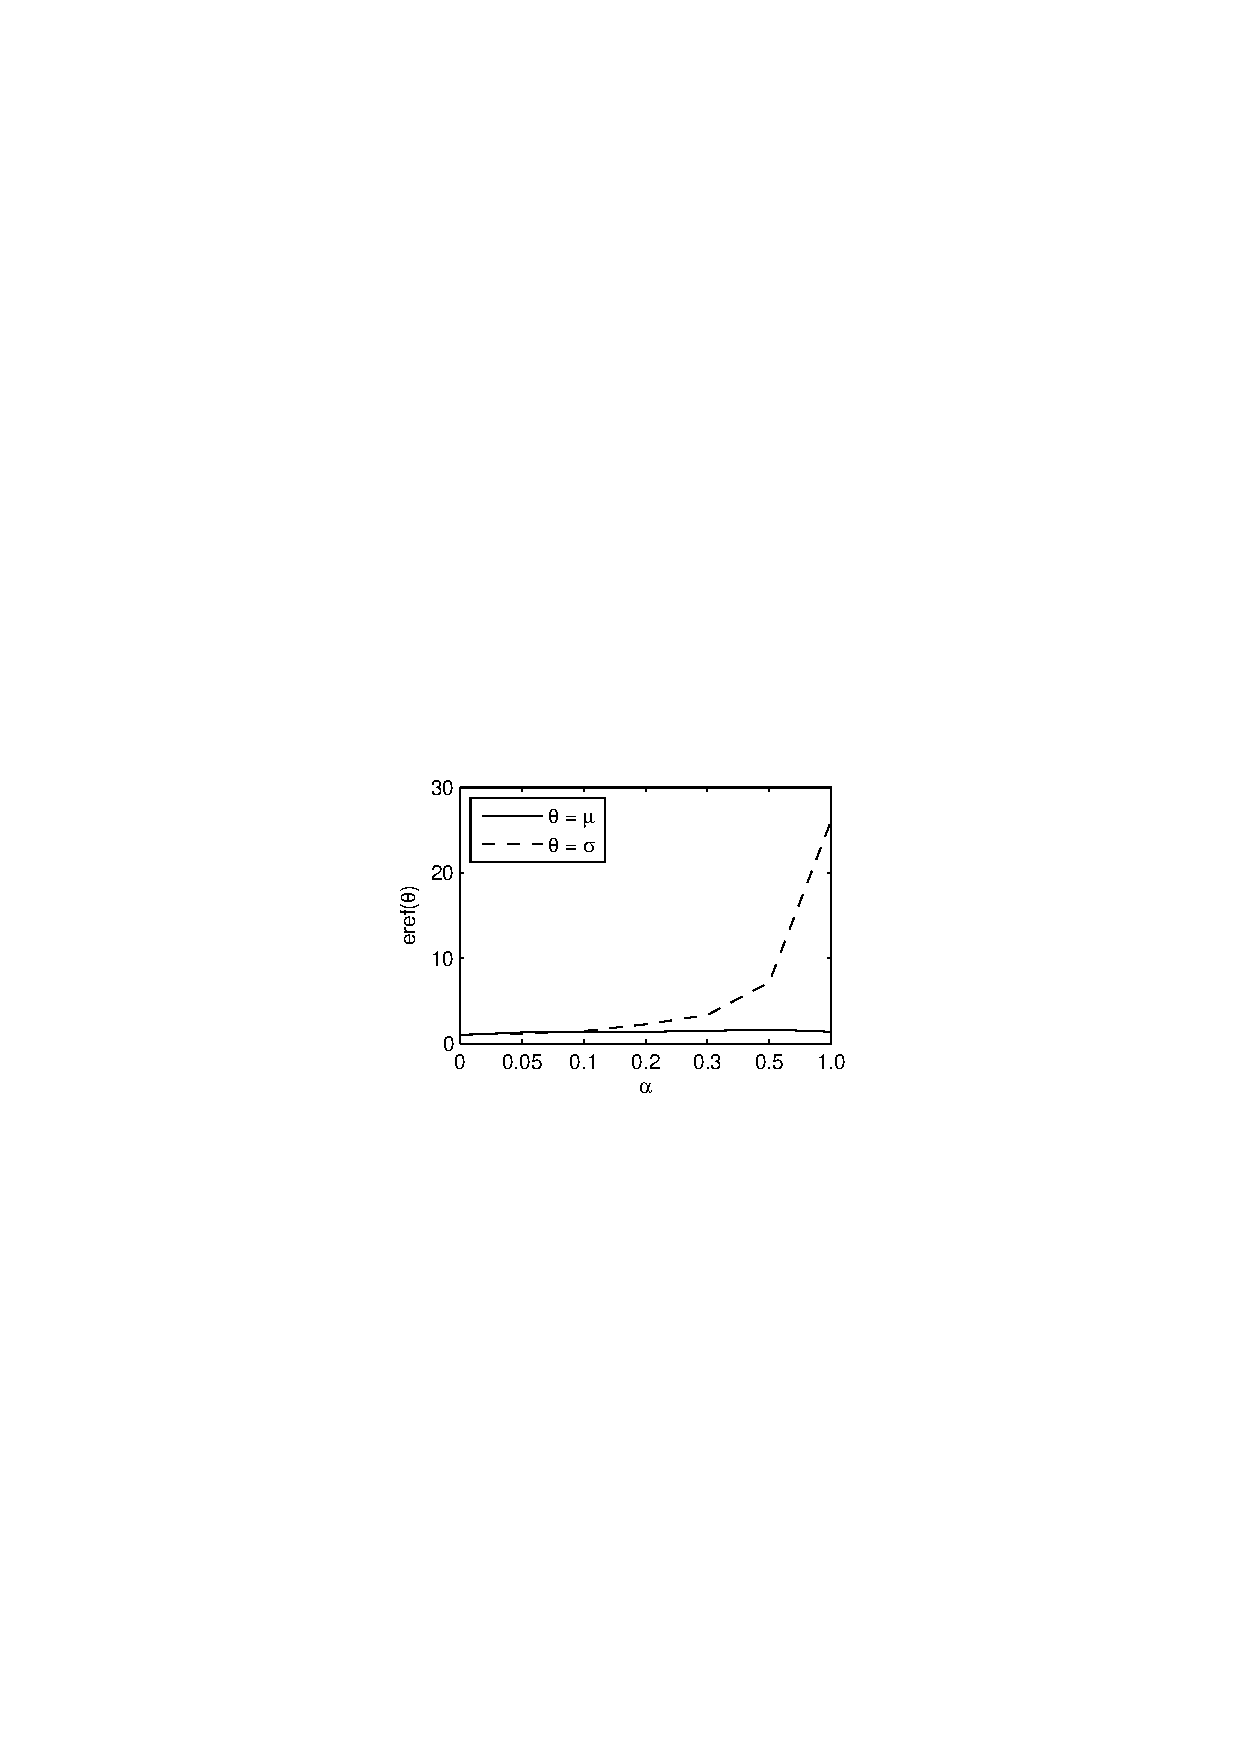
\includegraphics[width = 2in]{Cauchy-e04-eref.pdf}			
	\end{tabular}
\\
\end{tabular}
\end{center}
\caption{\footnotesize R\'{e}nyi: $p_\theta = \mathrm{C}(0,1)$, data: $(1-\varepsilon)\mathrm{C}(0,1) + \varepsilon \mathrm{C}(0,10)$, $\varepsilon =  0.4$}
%\label{tabJK:cauchy-eref}
\end{table}
\end{frame}


\begin{frame}
	\begin{figure}
		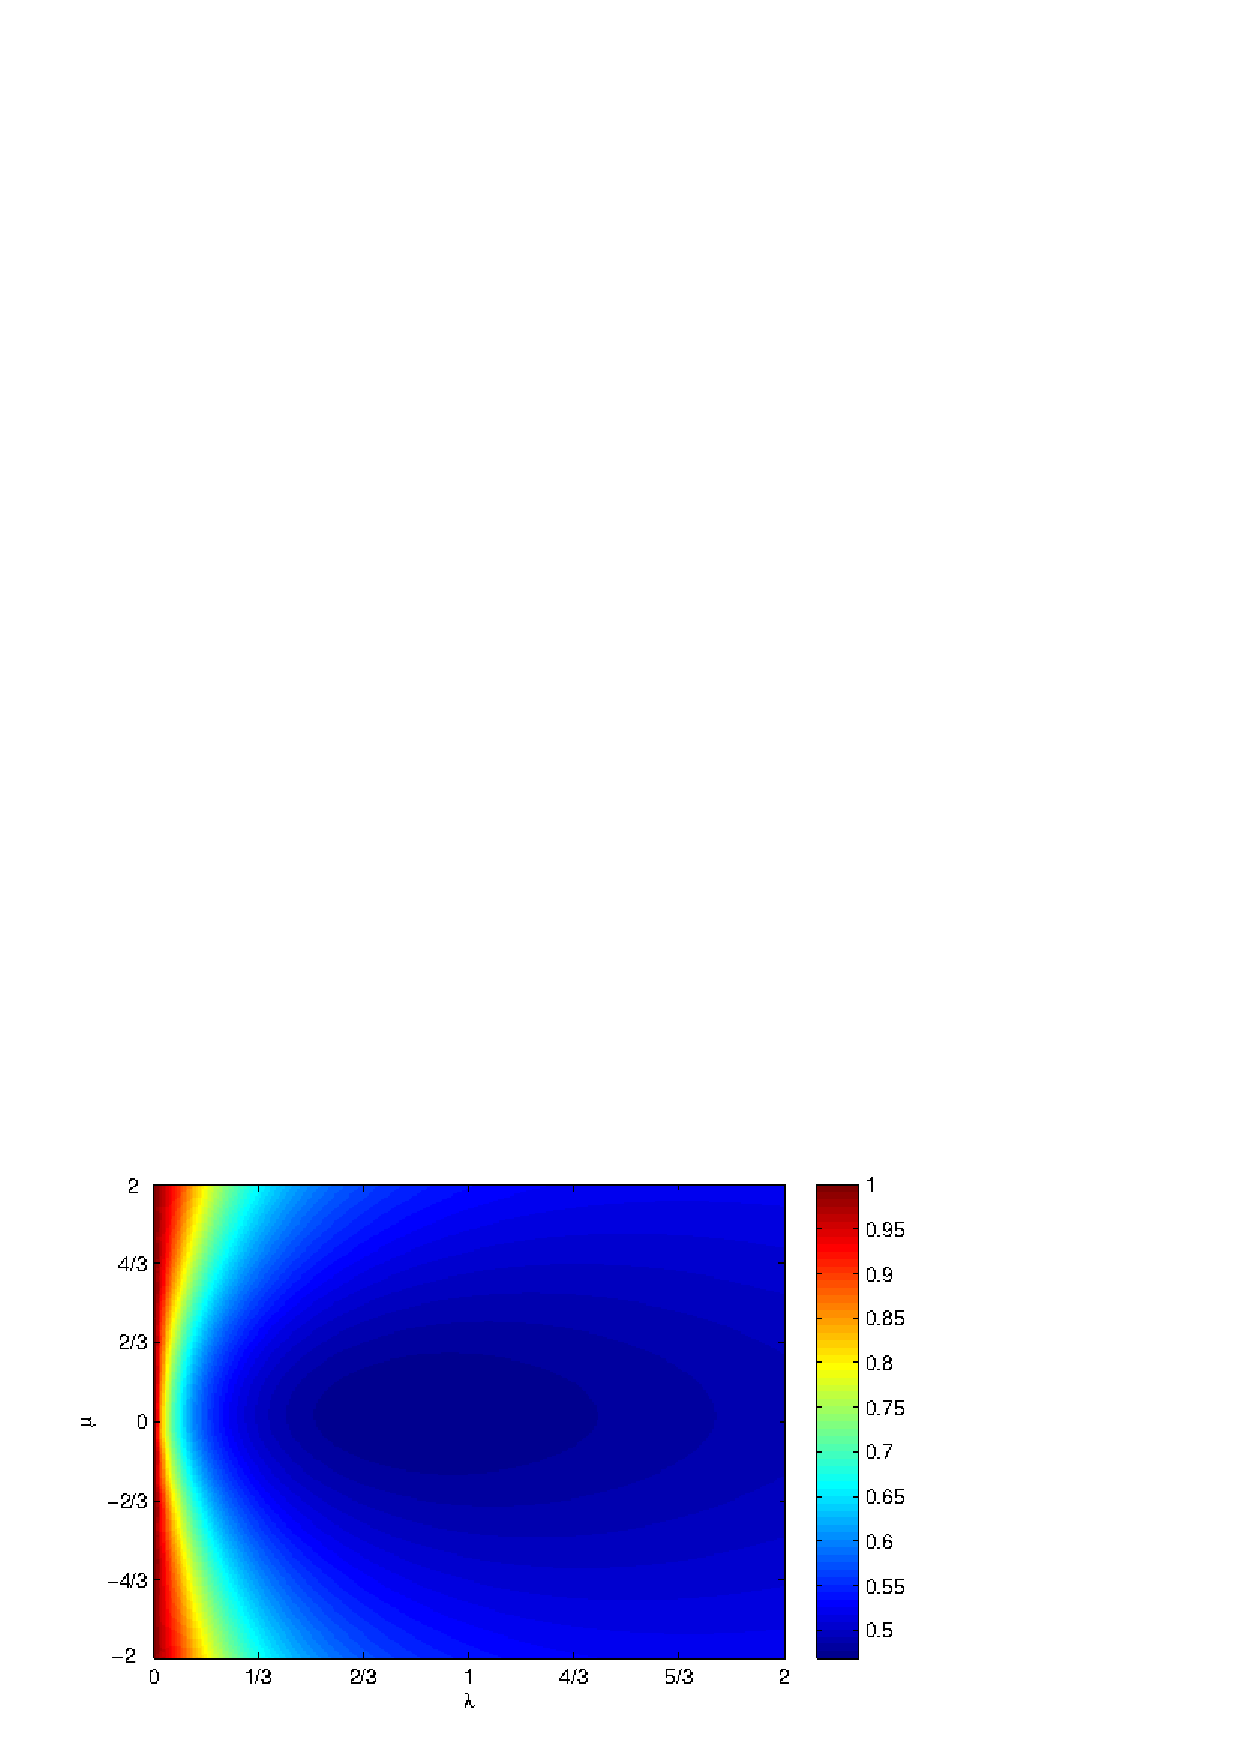
\includegraphics[width=2.5in]{L01-L010-distance-e03-a03_mark2.pdf}
		\caption{Rényiho pseudovzdálenost v Cauchyho modelu pro data tvořená jako směs $0.7\mathrm{C}(0,1) + 0.3\mathrm{C}(0,10)$, $\alpha = 0.3.$}
	\end{figure}
	\begin{itemize}
		\item globální minimum
		\item jednoduchá minimalizace pomocí algoritmů typu "hill climber"
	\end{itemize}
\end{frame}

\subsection{Laplaceovo rozdělení}    %%%%%%%%%%%%%%    LAPLACE    ********************************************************************************
%\begin{frame}{Laplaceovo rozdělení}
%
%{\footnotesize \[p_\theta = \frac{1}{2\lambda} e^{-\frac{|x-\mu|}{\lambda}},\qquad		\theta_{\mathfrak{R}_\alpha,n} = \amtiT (2\lambda)^{-\frac{\alpha}{1+\alpha}} \frac{1}{n} \sum_{i=1}^n \exp \left[-\alpha\frac{|x_i-\mu|}{\lambda} \right] \]}
%\begin{table}[htb] \tiny
%\begin{center}
%\begin{tabular}{ccc}
%	\begin{tabular}{|c|ccc|}
%	\hline
%	$\alpha\backslash n$ &&  $500$ & \\
%	\hline
%	& $m(\mu)$ & $s(\mu)$ & $eref(\mu)$ \\
%	& $m(\lambda)$ & $s(\lambda)$ & $eref(\lambda)$ \\
%	\hline
%	$0.0$ & $ -0.005 $ & $ 0.071 $ & $ 1.000 $\\
%	 & $ 4.593 $ & $ 3.617 $ & $ 1.000 $\\
%	\hline
%	$0.05$ & $ -0.000 $ & $ 0.071 $ & $ 1.018 $\\
%	 & $ 4.168 $ & $ 3.192 $ & $ 1.284 $\\
%	\hline
%	$0.1$ & $ 0.003 $ & $ 0.066 $ & $ 1.163 $\\
%	 & $ 3.719 $ & $ 2.741 $ & $ 1.742 $\\
%	\hline
%	$0.2$ & $ -0.002 $ & $ 0.068 $ & $ 1.098 $\\
%	 & $ 2.888 $ & $ 1.914 $ & $ 3.570 $\\
%	\hline
%	$0.3$ & $ -0.004 $ & $ 0.068 $ & $ 1.108 $\\
%	 & $ 2.215 $ & $ 1.241 $ & $ 8.490 $\\
%	\hline
%	$0.5$ & $ 0.001 $ & $ 0.069 $ & $ 1.056 $\\
%	 & $ 1.546 $ & $ 0.568 $ & $ 40.516 $\\
%	\hline
%	$1.0$ & $ 0.003 $ & $ 0.074 $ & $ 0.927 $\\
%	 & $ 1.221 $ & $ 0.256 $ & $ 199.663 $\\
%	\hline
%	\end{tabular}
%&&
%	\begin{tabular}{c}
%		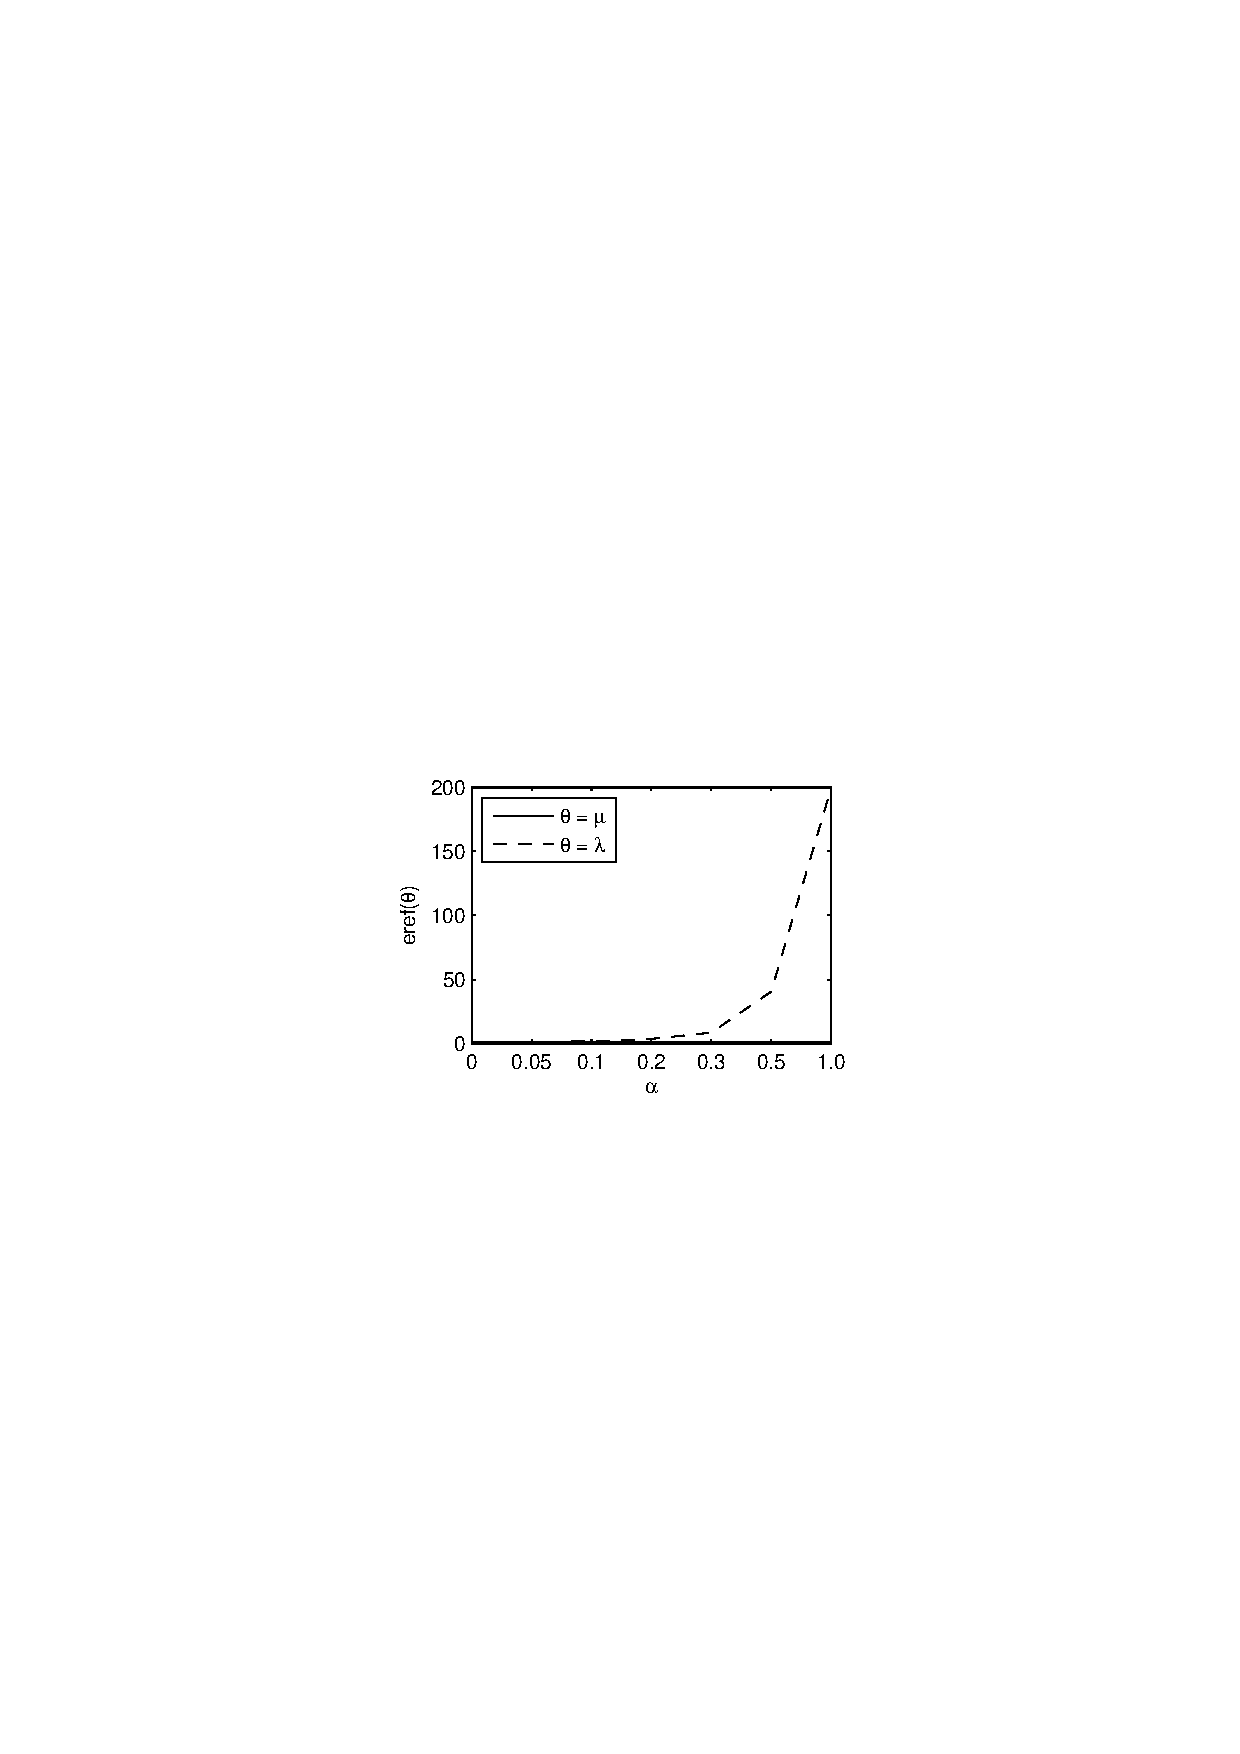
\includegraphics[width=2in]{Laplace-e04-eref.pdf}
%	\end{tabular}
%\\
%\end{tabular}
%\end{center}
%\caption{\footnotesize R\'{e}nyi: $p_\theta = \mathrm{L}(0,1)$, data: $(1-\varepsilon)\mathrm{L}(0,1) + \varepsilon \mathrm{L}(0,10)$, $\varepsilon =  0.4$}
%\label{tabJK:laplace-eref}
%\end{table}
%
%\end{frame}

\begin{frame}{Influenční funkce pro Laplaceovo rozdělení.}

{\footnotesize\[\mathrm{IF}(x;T_{\mathfrak{R}_\alpha},\mu) = (1+\alpha )^{\frac{3}{2}} (x-\mu )  e^{-\frac{\alpha}{2} (x-\mu )^2}\]}
{\footnotesize\[\mathrm{IF}(x;T_{\mathfrak{R}_\alpha},\lambda) = (1 + \alpha)^2 \left(-\lambda + (1 + \alpha)|x|\right)  e^{-\frac{\alpha|x|}{\lambda}}\]}
\vspace*{-0.3in}	
\begin{figure}[htb]
\begin{tabular}{lr}
	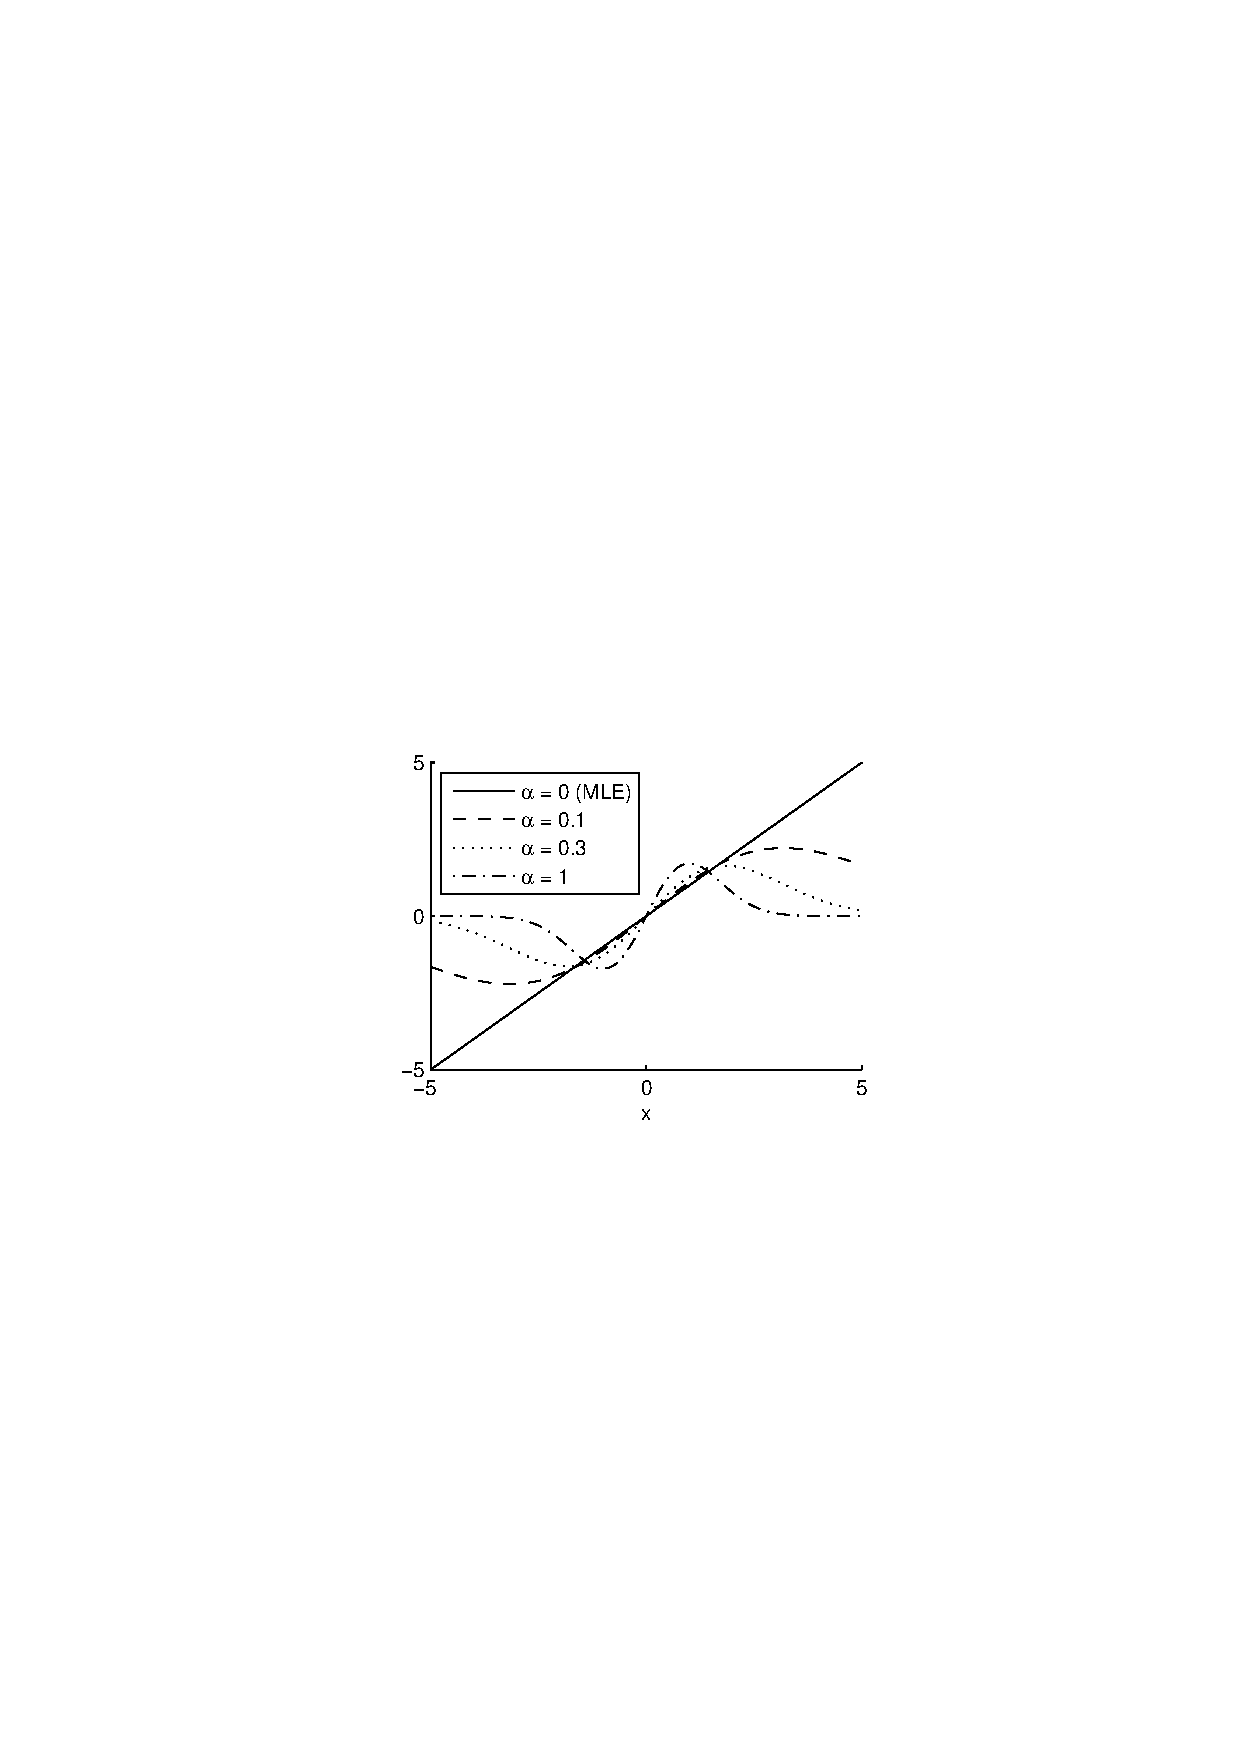
\includegraphics[width=1.7in]{Laplace-IF-mu.pdf}
	&
	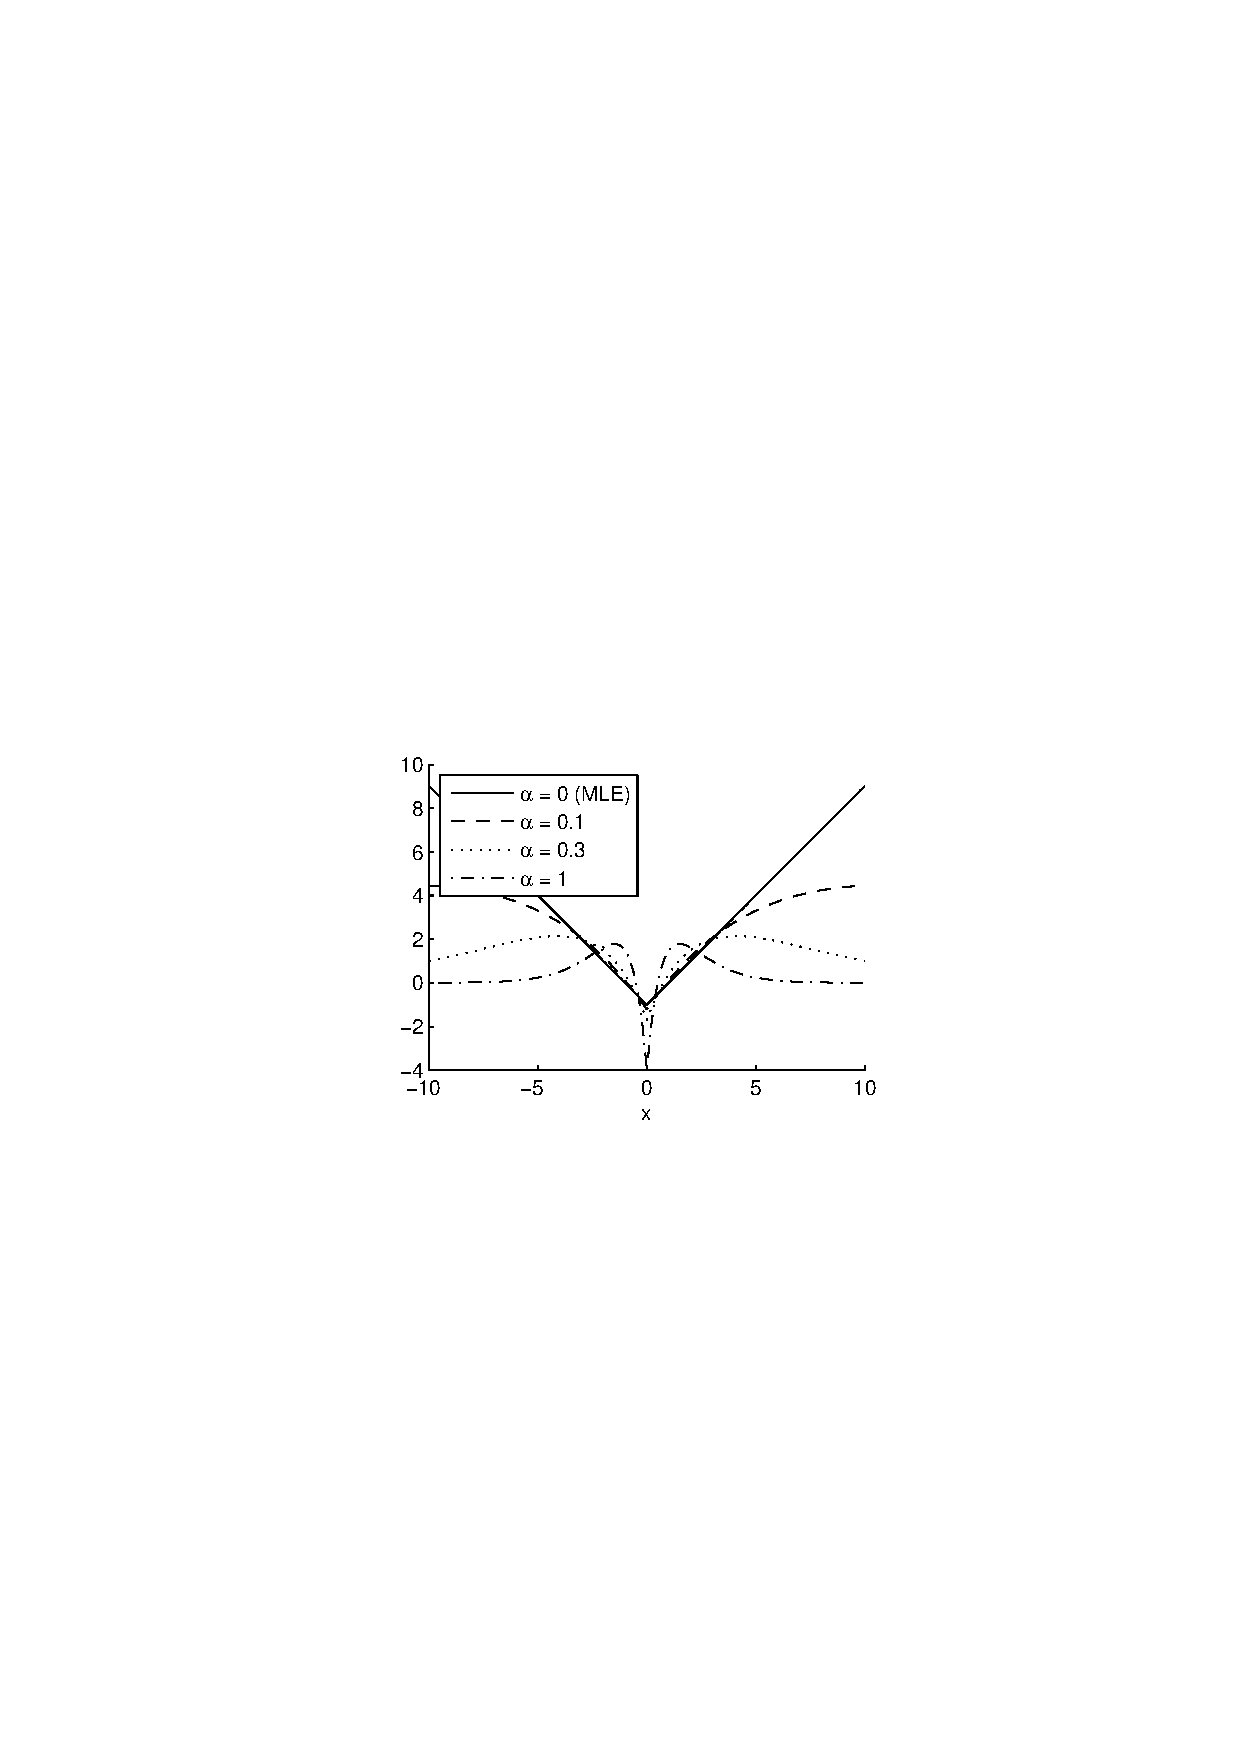
\includegraphics[width=1.7in]{Laplace-IF-lambda.pdf}
	\\
	{\footnotesize $\mathrm{IF}(x;T_{\mathfrak{R}_\alpha},\widehat{\mu} = 0) $, $\lambda = 1$}
	&
	{\footnotesize $\mathrm{IF}(x;T_{\mathfrak{R}_\alpha},\widehat{\lambda} = 1)$, $\mu = 0$}
	\\
\end{tabular}
\end{figure}
\vspace*{-0.1in}	
{\footnotesize Pro $\alpha> 0$}
\begin{itemize}
	\item {\footnotesize Omezené $\rightarrow$ B-robustní}
	\item {\footnotesize$\lim_{x\rightarrow \infty} \mathrm{IF}(x;T_{\mathfrak{R}_\alpha},\cdot) = 0 \; \rightarrow$ Robustní proti outlierům}
\end{itemize}


\end{frame}


\subsection{Exponencíální rozdělení}
\begin{frame}{Exponencíální rozdělení} %%%%%%%%%%%%%%%    EXPONENTIAL    *************************************************************************

{\footnotesize	\[ p_\theta = \frac{1}{\lambda} e^{-\frac{x-\mu}{\lambda}  }, \quad \theta_{\mathfrak{R}_\alpha,n} = \amtiT \lambda^{-\frac{\alpha}{1+\alpha}} \frac{1}{n}\sum_{i=1}^n \exp \left[-\alpha\frac{x_i-\mu}{\lambda} \right] \]}
\begin{table}[htb] \tiny
\begin{center}
\begin{tabular}{ccc}
	\begin{tabular}{|c|ccc|}
	\hline
	$\alpha\backslash n$ && $500$ & \\
	\hline
	& $m(\mu)$ & $s(\mu)$ & $eref(\mu)$ \\
	& $m(\lambda)$ & $s(\lambda)$ & $eref(\lambda)$ \\
	\hline
	$0.0$ & $ 0.003 $ & $ 0.004 $ & $ 1.000 $\\
	 & $ 4.659 $ & $ 3.683 $ & $ 1.000 $\\
	\hline
	$0.05$ & $ 0.003 $ & $ 0.005 $ & $ 0.951 $\\
	 & $ 4.184 $ & $ 3.207 $ & $ 1.319 $\\
	\hline
	$0.1$ & $ 0.003 $ & $ 0.004 $ & $ 1.070 $\\
	 & $ 3.738 $ & $ 2.761 $ & $ 1.780 $\\
	\hline
	$0.2$ & $ 0.003 $ & $ 0.005 $ & $ 0.932 $\\
	 & $ 2.887 $ & $ 1.911 $ & $ 3.712 $\\
	\hline
	$0.3$ & $ 0.003 $ & $ 0.004 $ & $ 1.005 $\\
	 & $ 2.196 $ & $ 1.224 $ & $ 9.057 $\\
	\hline
	$0.5$ & $ 0.003 $ & $ 0.005 $ & $ 0.738 $\\
	 & $ 1.545 $ & $ 0.569 $ & $ 41.931 $\\
	\hline
	$1.0$ & $ 0.007 $ & $ 0.012 $ & $ 0.145 $\\
	 & $ 1.217 $ & $ 0.255 $ & $ 208.991 $\\
	\hline
	\end{tabular}
&&
	\begin{tabular}{c}
		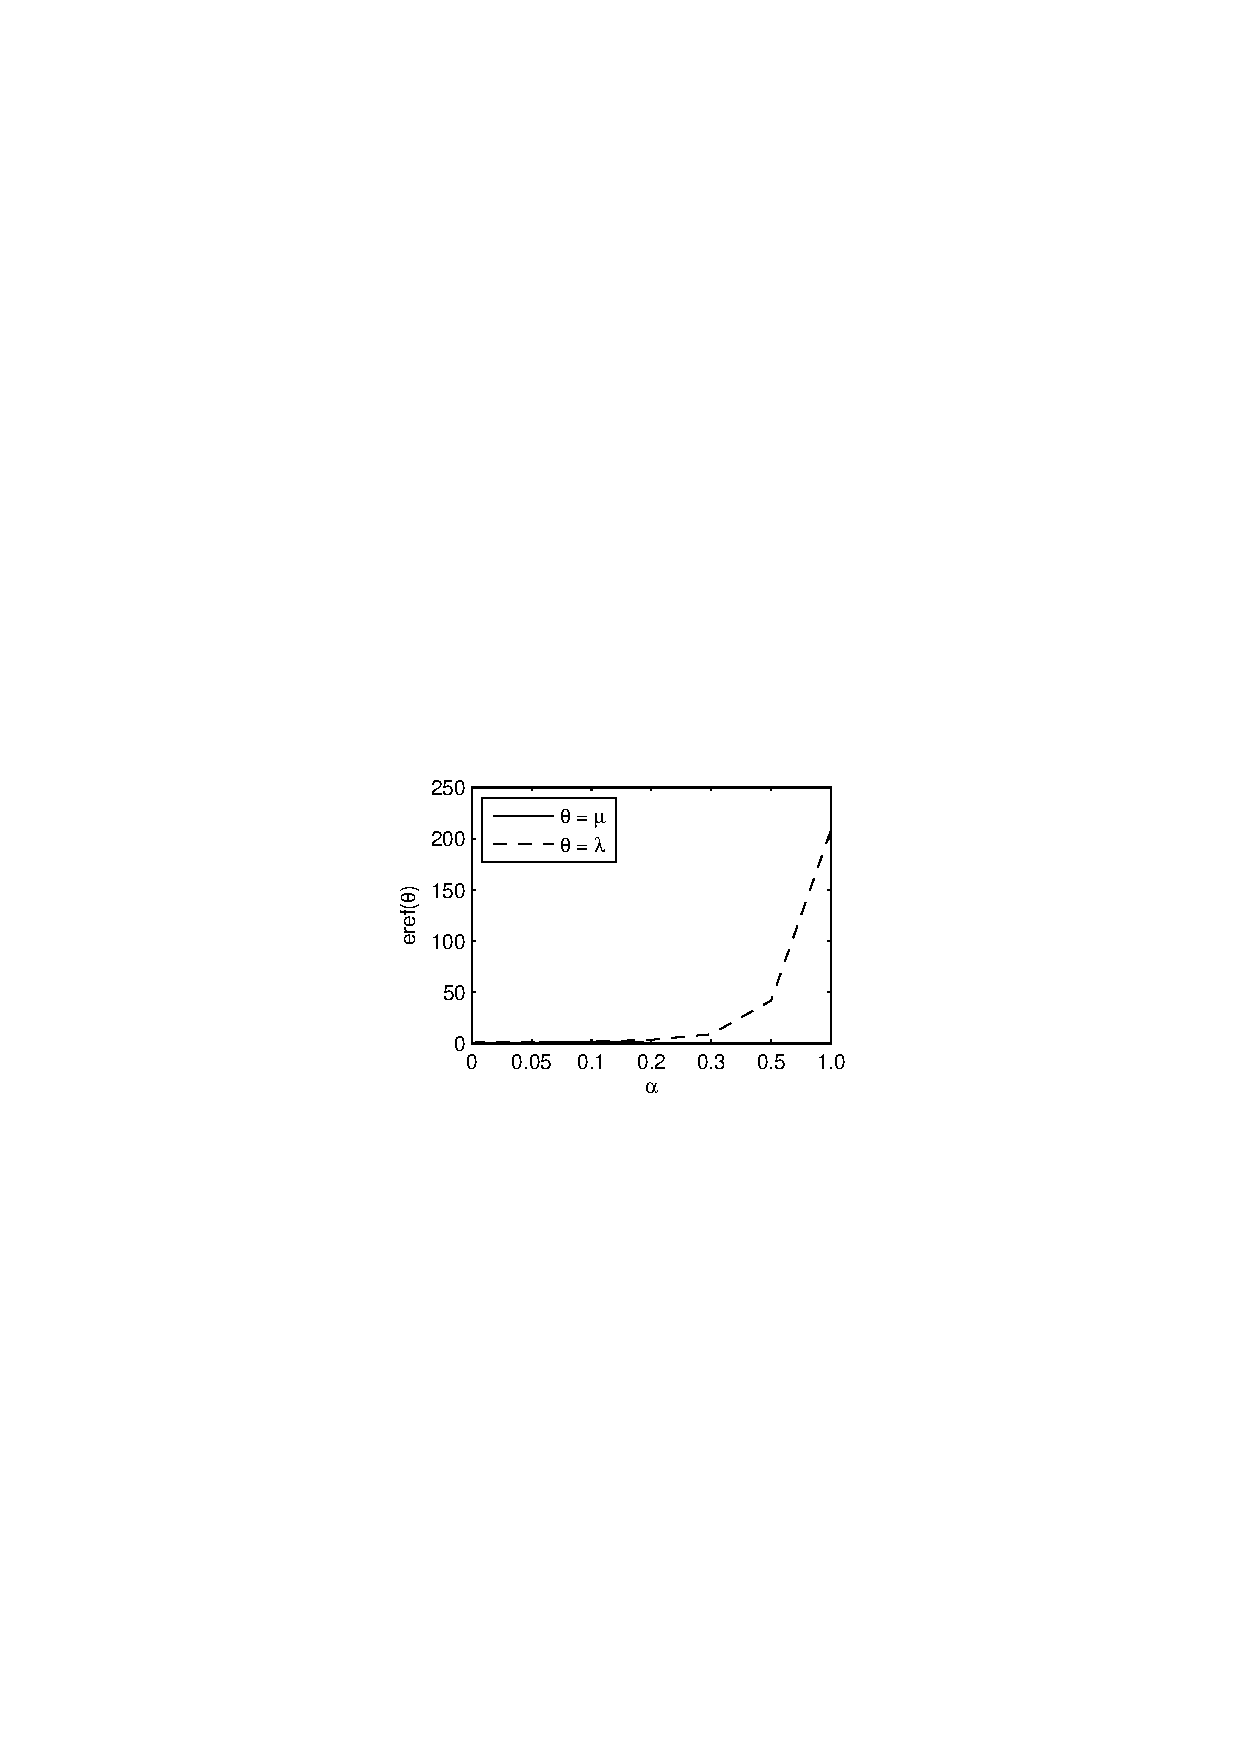
\includegraphics[width=2in]{Exp-e04-eref.pdf}
	\end{tabular}
\\
\end{tabular}
\end{center}
\caption{R\'{e}nyi: $p_\theta = \mathrm{E}(0,1)$, data: $(1-\varepsilon)\mathrm{E}(0,1) + \varepsilon \mathrm{E}(0,10)$, $\varepsilon =  0.4$.}
\label{tabJK:exponential-eref}
\end{table}	
\end{frame}

\begin{frame}
\begin{figure}
	\includegraphics[width=2in]{E01-E101-e05-a05-dist.pdf}	
	\caption{ Rényiho pseudovzdálenost v exponenciálním modelu pro data tvořená jako směs $0.5\mathrm{E}(0,1) + 0.5\mathrm{E}(10,1)$, $\alpha = 0.5.$}
\end{figure}
\begin{itemize}
	\item asymetrická vzdálenost 
	\item problém více lokálních extrémů
\end{itemize}
\end{frame}


%\begin{frame}
%	\begin{equation*}
%		\mathrm{IF}(x;T_{\mathfrak{R}_\alpha},\mu) = e^{-\frac{\alpha}{2} (x-\mu )^2} (1+\alpha )^{\frac{3}{2}} (x-\mu )
%	\end{equation*}
%	\begin{center}
%		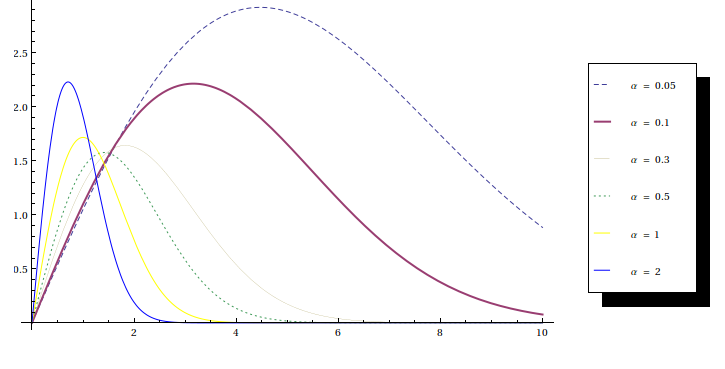
\includegraphics[width = 3.1in]{IF-Exponential-mu.png}			
%	\end{center}
%\end{frame}
%
%\begin{frame}
%	\begin{equation*}
%		\mathrm{IF}(x;T_{\mathfrak{R}_\alpha},\lambda) =	(1+\alpha )^2 ( - \lambda +(1+ \alpha)x) e^{-\frac{\alpha x}{\lambda }}
%	\end{equation*}
%	\begin{center}
%		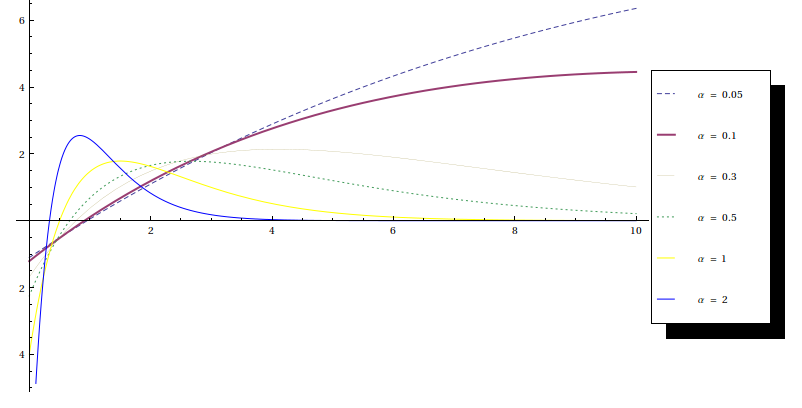
\includegraphics[width = 3.1in]{IF-Exponential-sigma.png}			
%	\end{center}
%\end{frame}
%
%\begin{frame}
%\begin{table}[ht] \footnotesize
%\begin{center} 
%\begin{tabular}{|c|ccc|} 
%\hline 
%$\alpha\backslash n$ && $500$ & \\ 
%\hline 
%& $m(\lambda)$ & $s(\lambda)$ & $eref(\lambda)$ \\ 
%\hline 
%$0.0$ & $ 3.901 $ & $ 0.432 $ & $ 1.000 $\\ 
%\hline 
%$0.01$ &$ 3.614 $ & $ 0.356 $ & $ 1.475 $\\ 
%\hline 
%$0.05$ & $ 3.241 $ & $ 0.317 $ & $ 1.862 $\\ 
%\hline 
%$0.1$ & $ 2.796 $ & $ 0.274 $ & $ 2.495 $\\ 
%\hline 
%$0.15$ & $ 2.389 $ & $ 0.239 $ & $ 3.258 $\\ 
%\hline 
%$0.2$ &$ 2.049 $ & $ 0.209 $ & $ 4.281 $\\ 
%\hline 
%$0.3$ & $ 1.622 $ & $ 0.153 $ & $ 7.999 $\\ 
%\hline 
%$0.5$ &  $ 1.310 $ & $ 0.110 $ & $ 15.330 $\\ 
%\hline 
%$1.0$ &  $ 1.139 $ & $ 0.109 $ & $ 15.806 $\\ 
%\hline 
%\end{tabular}
%\caption{Renyi: $p = \mathrm{E}(0,1)$, data: $(1-\varepsilon)\mathrm{E}(0,1) + \varepsilon \mathrm{E}(0,10)$, $\varepsilon =  0.3$, $K = 1000$} 
%\end{center}
%\end{table}
%\end{frame}

%\subsection{Weibullovo rozdělení}
%\begin{frame}{Weibullovo rozdělení} %%%%%%%%%%%%%%     WEIBULL     *******************************************************
%	\begin{equation*}
%		p_\theta =  \frac{k}{\lambda} \left( \frac{x-\mu}{\lambda} \right)^{k-1} \exp \left[ -\left( \frac{x-\mu}{\lambda} \right)^k \right] 
%	\end{equation*}
%	\begin{eqnarray}
%		\theta_{\mathfrak{R}_\alpha,n} & = & \amtiT \left( \frac{k}{\lambda} \right)^\fa (1+\alpha)^{\fa\frac{1+\alpha+k}{k}} \Gamma\left(\frac{1+\alpha+k}{k}\right)^{-\fa} \nonumber \\
%							&& \frac{1}{n}\sum_{i=1}^n \left( \frac{x_i-\mu}{\lambda}\right)^{\alpha(k-1)} \exp\left[-\alpha \left(\frac{x_i-\mu}{\lambda}\right)^k\right] \nonumber
%	\end{eqnarray}
%\end{frame}
%
%%\begin{frame}
%\begin{table}[ht] \footnotesize 
%\begin{center} 
%\begin{tabular}{cc}
%\begin{tabular}{|c|ccc|} 
%\hline 
%$\alpha\backslash n$ &&  $500$ & \\ 
%\hline 
%& $m(\lambda)$ & $s(\lambda)$ & $eref(\lambda)$ \\ 
%\hline 
%$0.0$ & $ 4.713 $ & $ 0.387 $ & $ 1.000 $\\ 
%\hline 
%$0.01$ & $ 4.568 $ & $ 0.364 $ & $ 1.130 $\\ 
%\hline 
%$0.05$ & $ 4.149 $ & $ 0.373 $ & $ 1.077 $\\ 
%\hline 
%$0.1$ &$ 3.511 $ & $ 0.383 $ & $ 1.020 $\\ 
%\hline 
%$0.15$ & $ 2.574 $ & $ 0.428 $ & $ 0.815 $\\ 
%\hline 
%$0.2$ & $ 1.664 $ & $ 0.261 $ & $ 2.201 $\\ 
%\hline 
%$0.3$ &  $ 1.226 $ & $ 0.076 $ & $ 25.766 $\\ 
%\hline 
%$0.5$ & $ 1.096 $ & $ 0.057 $ & $ 46.725 $\\ 
%\hline 
%$1.0$ & $ 1.043 $ & $ 0.055 $ & $ 49.962 $\\ 
%\hline 
%\end{tabular}
%&
%\end{tabular}
%\caption{Renyi: $p = \mathrm{W}(1.5,1)$, data: $(1-\varepsilon)\mathrm{W}(1.5,1) + \varepsilon \mathrm{W}(1.5,10)$, $\varepsilon =  0.3$, $K = 1000$} 
%\end{center}
%\end{table}
%\end{frame}
%
\section{}
\begin{frame}{Shrnutí}
	Rényiho pseudovzdálenosti
	\begin{itemize}
		\item B-robustní		
		\item robustní vůči outlierům
  		\item poměrně jednoduše minimalizovatelná funkce
		
	\end{itemize}
\end{frame}



\begin{frame}
	\begin{center}
		Děkuji za pozornost.
	\end{center}
\end{frame}

\end{document}


























